% Chapter 2

\section{Introducing Discite}

Discite is a web application that belongs to the MOOC domain (Massive Open
Online Course).  It's based around the idea of interactivity, the main features
being a synchronized slideshow, and audio/video broadcast, that were implemented with
Server Sent Events and WebRTC. The application is based on web technology because of ease
of development, good abstractions, and hassle-free cross-platform support.

\subsection{Feature overview}
% accounts, presentation, chat, video/audio
Discite provides a web-based implementation of a new way to have peer-to-peer
lessons, using open standards, based on cutting-edge technology, mainly HTML5,
and features that are still in development, and process of standardization.

The web sites requires authentication to work. Only a minimum of information is collected.
The only required attributes are email and password. A user name can be provided optionally, if not, then the
first chunk of the email is used instead. After an account is created, a profile
page can be accessed, where one can change the password, choose a preferred
language for the website, as shown in Figure~\ref{fig:edit_profile}.
\begin{figure}[ht!]
\centering
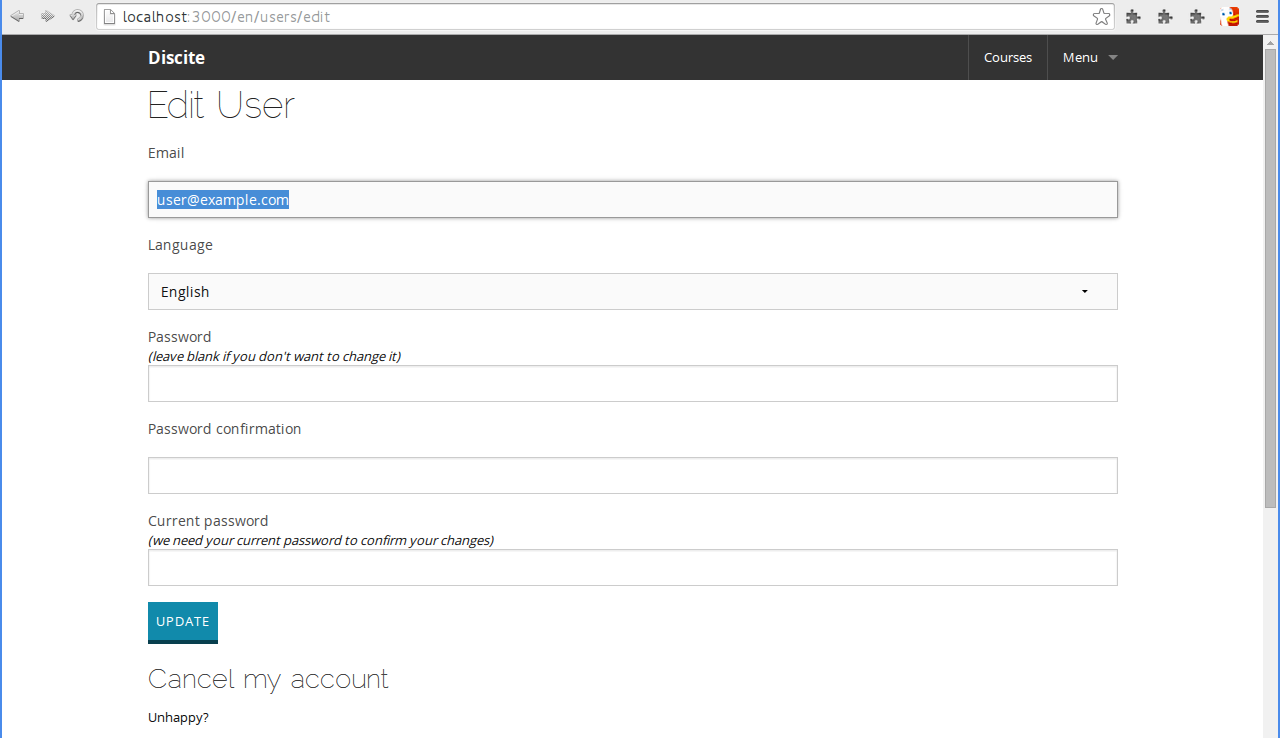
\includegraphics[width=\textwidth]{edit_profile}
\caption{Edit profile page}
\label{fig:edit_profile}
\end{figure}
Also, a useful feature is that not only teachers can create courses (there is no concept
of a teacher at the application level, there are just course owners), and anyone
can see what teaching implies, and spread their skills to a wide audience. For
the time being, the courses are shown in a list, presented in Figure~\ref{fig:course_list}.
\begin{figure}[ht!]
\centering
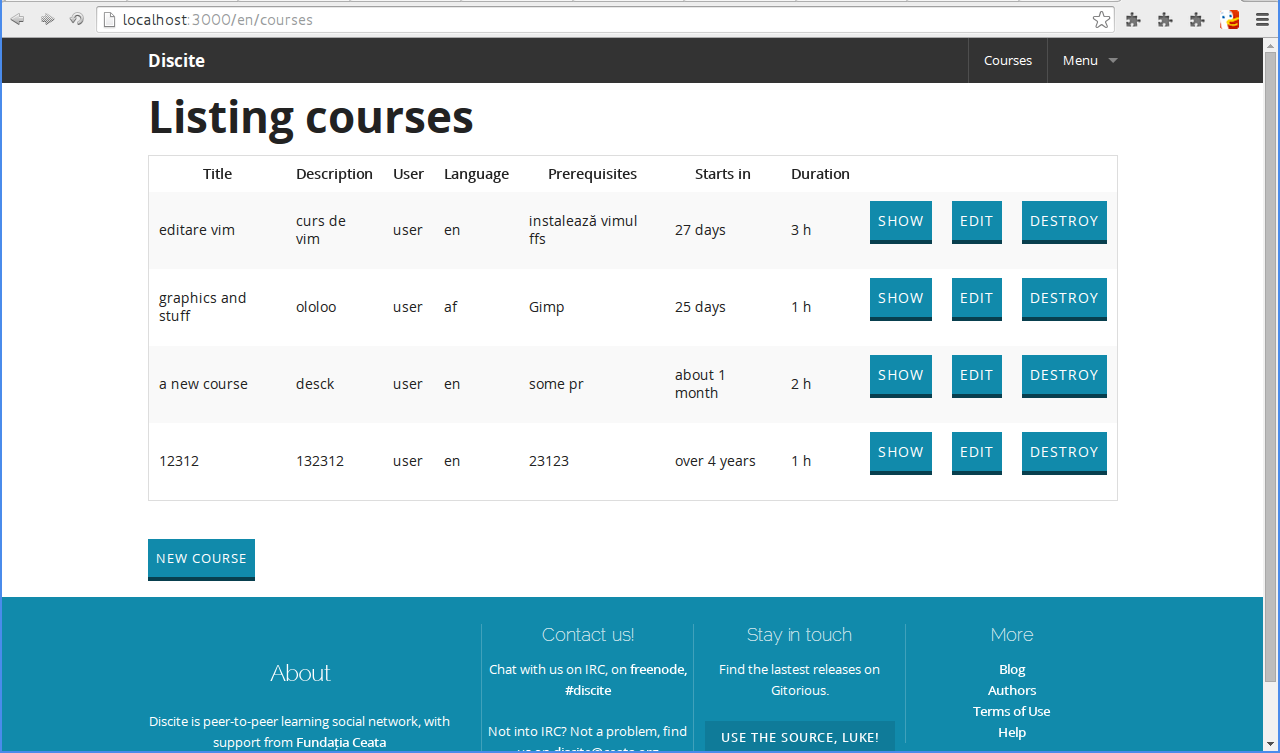
\includegraphics[width=\textwidth]{course_list}
\caption{Course list page}
\label{fig:course_list}
\end{figure}
One of the main features is the synchronized slideshow, as shown in Figure~\ref{fig:slideshow}.
The slideshow is controlled by the teacher, and are
synchronized by the application server, which uses Server Sent Events to notify
the other clients of slide changes.

While it's possible to spawn a menu (by
pressing "G") to switch to any page the teacher wishes, currently only the
next and previous slide events are synchronized. Synchronization for other types
of events is planned in future versions.
\begin{figure}[ht!]
\centering
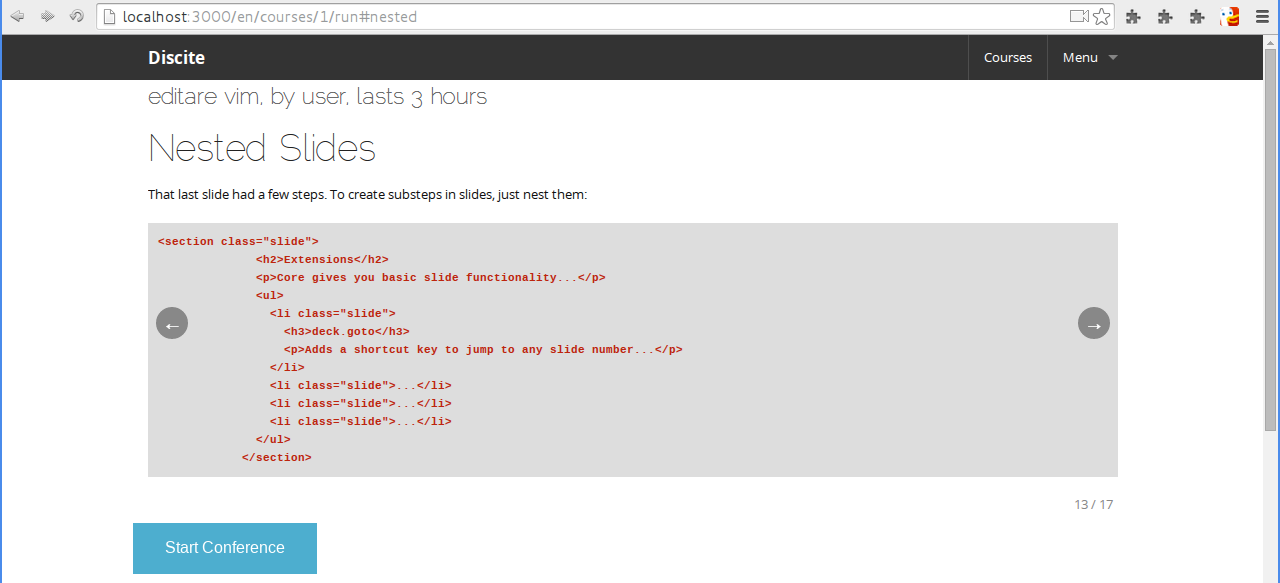
\includegraphics[width=\textwidth]{slideshow}
\caption{Running course page}
\label{fig:slideshow}
\end{figure}
The other core feature is the video conference, a demonstration of which is shown in Figure~\ref{fig:conference}.
This is possible due to recent development in
the standardization of WebRTC (Web Real Time Communication), that is already
implemented in several major browsers, namely Chromium and Firefox.  WebRCT is a
collection of standards, protocols, and JavaScript APIs, the combination of
which enables peer-to-peer audio, video, and data sharing between browsers
(peers). Instead of relying on third-party plug-ins or proprietary software,
WebRTC turns real-time communication into a standard feature that any web
application can leverage via a simple JavaScript API.
\begin{figure}[ht!]
\centering
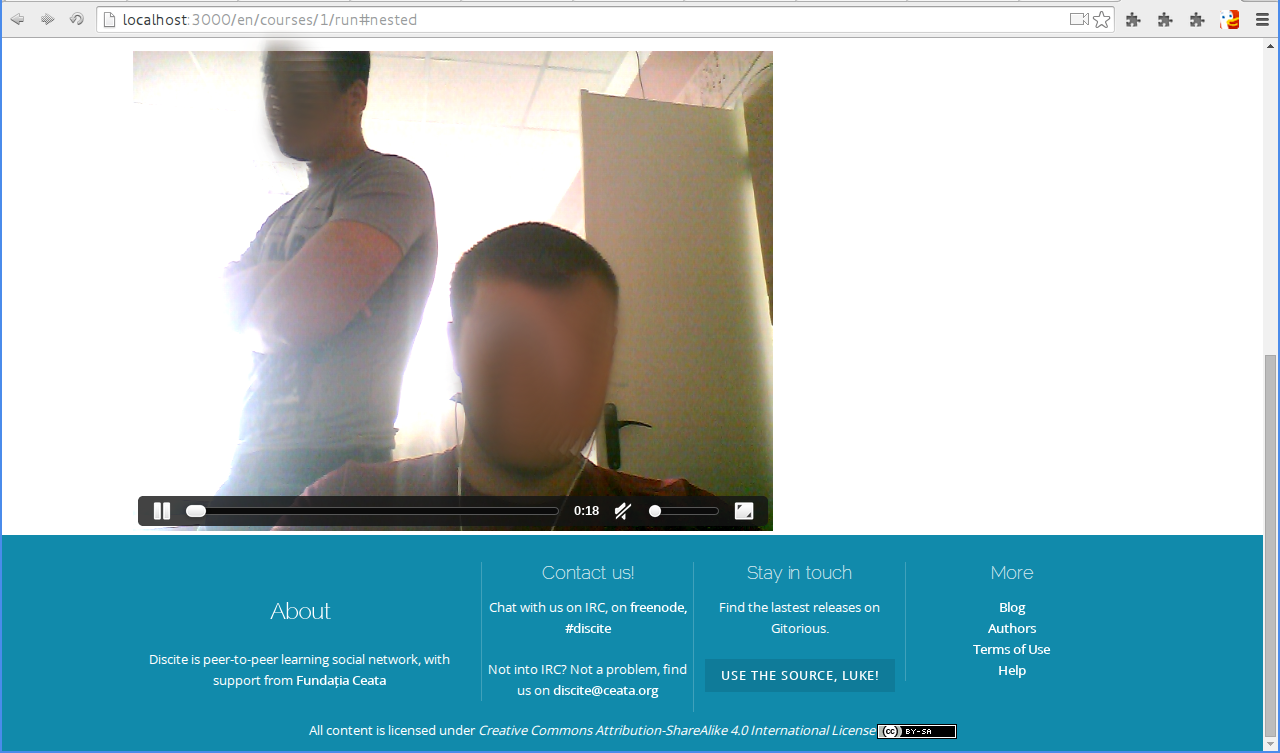
\includegraphics[width=\textwidth]{conference}
\caption{Video broadcasting view}
\label{fig:conference}
\end{figure}

Initially there was a large list of planned features (most of which are implemented already), but as it
turns out some of them were not possible to implement due to technical reasons, and others because they
conflicted with other system features, or with the user experience. Those features planned originally are:
\begin{enumerate}[topsep=5pt, partopsep=0pt,itemsep=3pt,parsep=1pt]
    \item[--] pick a course based on your interests
    \item[--] give the course and teacher a rating
    \item[--] choose a preferred language
    \item[--] filter by skills one is looking for
    \item[--] screen sharing
    \item[--] voice/videochat
    \item[--] presentation
    \item[--] doodling
\end{enumerate}

The use-case diagram presented in Figure~\ref{fig:use_case} provides a higher-level view of the system,
and what is the flow of work and interaction with Discite.
\begin{figure}[ht!]
    \centering
    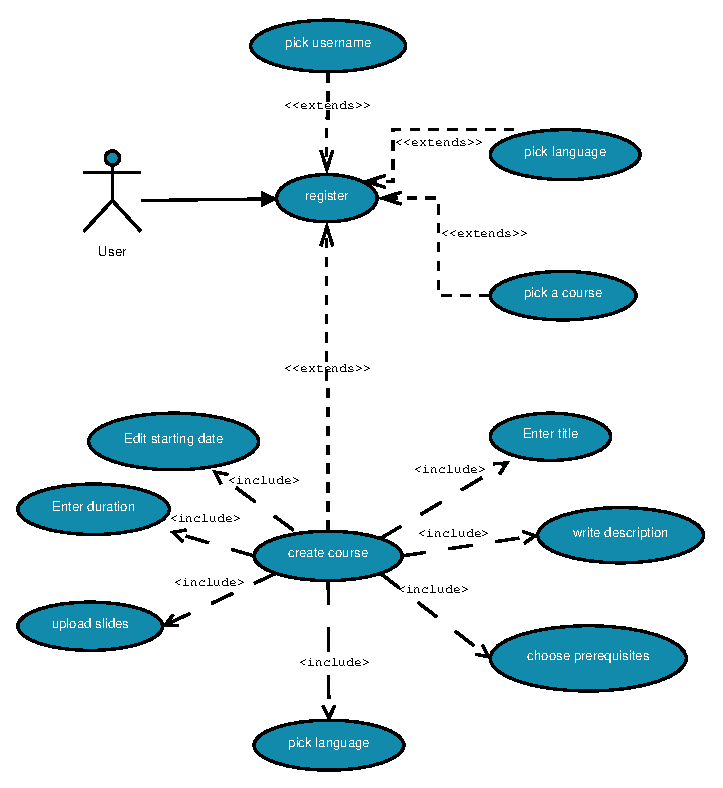
\includegraphics[height=13cm]{use_case}
    \caption{Use case diagram}
    \label{fig:use_case}
\end{figure}
These features make the system very interactive, as all actions are propagated
nearly in real-time, and it brings some of life proved teaching techniques,
where a student can interrupt and change the way a lesson goes.  Teacher and
students can alter the way a course goes, they can interact by chat,
doodling.  On the down side, the teacher and students have to meet at a
certain time. The course recordings can be watched after that, but that wont
bring the aforementioned benefits.
% 4 pages
\subsection{Use within the classroom}
The application can be used complementary to
the traditional way of teaching, as e-learning has been underrated at the
college level, and that some of its methods and techniques can augment
traditional classroom learning.  Students today are surrounded by technology -
it is part of their normal life style. Teachers need to make the world reflect
the optimization school environment for our students. Educators need to bridge
the gap between busy teachers and students that are accustomed with technology,
and this is easily achievable with a MOOC platform.  The presentation module
present in Discite can be exploited successfully in the classroom, as it's
common nowadays for students to bring their own devices to school, be it
laptops, or tablets, an for those who don't, the classrooms become more and more
featured with digital equipment, and they can be used to sustain the digital
learning process.  This blend of two worlds is a more learner-friendly
alternative, as the teacher becomes more of a facilitator than a teacher.

“Not only does that enhance the collaborative nature of online learning, it also
motivates students to be much more engaged and to take more responsibility for
what they’re learning” as Haythornthwaite from the Illinois Univsity puts it
\citep{haythornthwaite}.

However much e-learning may reshape education, it’s not necessarily meant to
supplant classroom learning, but is more of a supplement to it.
Massachusetts Institute of Technology for example put all of its classroom
materials online for non-commercial use in 2001, as an example of how “blended
learning” can be created from a mixture of e-learning and classroom interaction.

On the other hand, the equipment is quite expensive, and it's outdated at very
fast rates these days. And sometimes the students get distracted by the gizmo,
which may hinder the educational process
% 2 pages
\subsection{Online usage} Mixing technology and leaning can lead to very powerful
ways of teaching, that were previously impossible. Think of the suggestive
animations, of embedded videos inside a web page, 3D models, simulations: all
available to make the new material not only easily digestible, but also highly
interactive and even addictive. This was exploited very successfully in online
games, and people are spending huge amounts of time on them, learning the
virtual environment, making virtual friends, and having virtual social
interaction.  Discite builds a more real connection between teacher and student,
because they can see their teacher, which raises engagement in the learning
activity.  The real time nature of the process creates a medium for deeper
interaction, as the student doesn't have time to become distracted. The teaching
process also becomes more personal and fast, and more commitment is expected to
be shown from students.
Making a course is fast, usually taking around half an hour, and uses a specially
crafted interface, shown in Figure \ref{fig:course_creation}.
\begin{figure}[ht!]
\centering
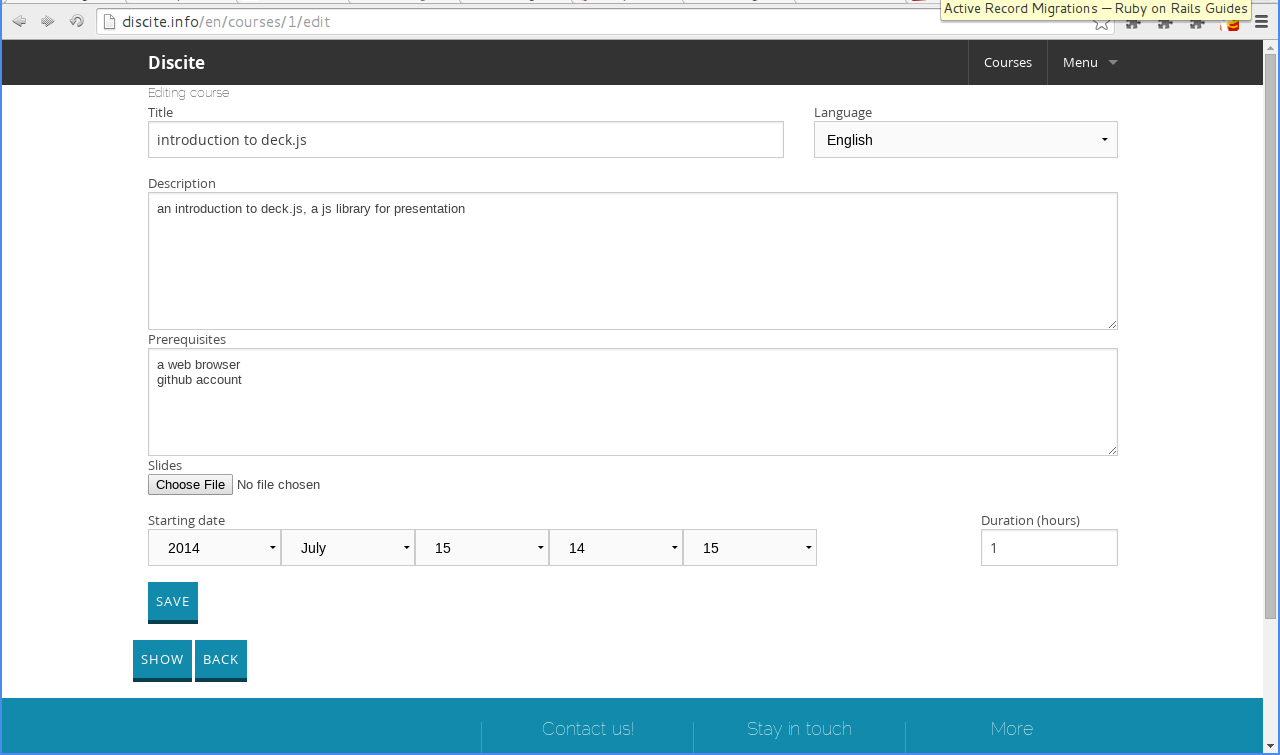
\includegraphics[width=\textwidth]{course_creation}
\caption{Form for course creation}
\label{fig:course_creation}
\end{figure}
\\
The time to build a course is not fixed, of course, and it depends on it's complexity
and the skills of the one who is building it.

There are of course problems with the online usage of Discite: time zones become
a concern, and sometimes students and teachers can't find a optimum time to meet
each other. When compared to the regular approach to MOOC, more time is wasted:
the same lesson has to be held again for another group of students, or another
generation.  As a correction for this kind of bad behavior, Discite can be used
as a complementary tool, used to deliver only critical courses, and a more
asynchronous way of e-learning can be employed, to cope with the busyness of
people schedules.

In conjunction with evaluation of needs, e-learning can target specific needs,
and by using learning style tests, e-learning can  target individual learning
preferences.  Additionally, asynchronous e-learning is self-paced. Advanced
learners are allowed to speed through or skip instruction that is redundant
while novices slow their pace through content, alleviating frustration with
their progress, their fellow, and the course.  This way, e-learning is allowing
inclusion of a large number of participants with a maxed out range of learning
styles, preferences, and needs.  Consistent delivery of content is possible with
asynchronous style of courses, and also with Discite presentation system. As a
feature to be implemented in the future is recordings of a course, or even
archival, full with comments, video, slides, and chat.  Expert knowledge is
communicated and captured inside the system, if the system is good enough, and
take care to allow storing it easily, an retrieving it without difficulty from
the e-learing and knowledge system.  Proof of completion and certification, as
central elements of training initiatives, while not in the scope of the current
system can be implemented.  There are other advantages for the learners, by
going online and using Discite: increased information retention, reduced
learning time, on-demand availability that enables students to complete training
conveniently at any time they desire, giving them flexibility.  Interactivity
engages users, pushing them rather than pulling them through the learning
process. The fact that quick reference materials are available reduces the
worrying associated with responsibility of mastering a particular skill.

There are some pain points about doing lessons online on the Dicite
platform, like the time invested for rewriting presentations in HTML.
Also, technology issues could play a role as sometimes existing technology
infrastructure can fulfill the training goals, and additional
expenditures cannot be justified. This might be the case if Technical University of Moldova
 were to switch from Moodle to Discite. One more issue that may arise is
 cultural acceptance as in some organizations the students/trainees demographics may be
 against using a computers, let alone to learn using one.
% 3 pages
\subsection{Freedom and extensibility} The application is licensed under AGPLv3,
and the code is available on Github and Gitorious for download. Universities or
companies can use it to build on top of it, or they can contract programmers to
extend the program, and they can peer review it. Other developers can reduce the
complexity and improve the maintainability of software. This rarely comes high
on the product plan for proprietary software. Third parties can also inspect the
code,find bugs, or add critical features for their narrow scope, and if that is
a small niche, it could never be achievable in another way.

Discite also offers business flexibility, so that as requirements in the
business change, solutions should not be unreasonably constrained by software.
This is especially important in the area of infrastructure components — the
architecture of the IT solution as Discite might be.  Business users are most
likely to obtain long-term flexibility through the careful choice of standards
for data exchange, followed by enough care  to ensure that freedom from
proprietary lock-in is maintained. The drawback is that standards sometimes lack
in terms of shiny features. Discite is strong in this area, not only from the
point of view of following standards but also by helping to mitigate against
insidious lock-in if it is used a core infrastructure component.

Software vendors can go out of business, or they can decide to cease
development of a product, but as the source is available, the risk is not that
imminent with Discite. Our users not only have  the right to use the software
they already have, but the ability to continue to use it as their needs change.
The project has a open IRC channel, on the freenode network, \#discite - question
about development ideas, or what various components do can be asked there.

% 1 page
\subsection{Acessibility and Internationalization} In creating the Discite
platform, special care was put in user experience. \textit{Zurb Foundation} was chosen
as the basis of the application interface. It has already implemented most usual
widgets, such as buttons, forms, headers, menu.  Also, inspiration was taken
from various sources, including interface guidelines.

The most important and complicated page in the whole system is the course page.
The idea was initially to have a page split in four: the video chat, the text
chat, the presentation and the doodling area, but after toying with this idea,
the decision was to keep it more simple, with presentation on top, and with the
video conference at bottom. A side panel for chat will be implemented in later
versions.

Also, attention was given to accessibility, which  means that people with
disabilities can use the application. Web accessibility benefits not only disabled people,
but other groups too, like older people with changing abilities due to aging.
The Web is an more and more important resource in many aspects of life: education,
employment, government, commerce, health care, recreation, and more. It's of great
importance that Discite is accessible in order to provide equal access and equal
opportunity to people with disabilities. An accessible Web can also help people
with disabilities to participate more actively in society, and the learning process
Discite provides.

